\clearpage
\setcounter{page}{1}
\setcounter{section}{0} % 重置章节计数器
\renewcommand{\thesection}{\Alph{section}} % 将章节编号改为字母形式

\maketitlesupplementary

\section{Additional Experimental Results}
\label{app:additional_experiment_results}
\begin{table*}[htbp]
    \centering
    \caption{\textbf{Full result on MME-RealWorld-Lite.}}
    \label{tab:mme_full}
    \resizebox{0.9\textwidth}{!}{%
    \begin{tabular}{lccccc|cccccc}
        \hline
        & \multicolumn{11}{c}{\textbf{MME-RealWorld-Lite}} \\
        \cmidrule{2-12}
        & \multicolumn{5}{c}{\textbf{Reasoning}} & \multicolumn{6}{c}{\textbf{Perception}} \\
        \cmidrule{2-6} \cmidrule{7-12}
        & Overall & MO & AD & OCR & DT & overall & MO & AD & OCR & DT & RS  \\
        \hline
        %GPT-4o & 37.61 & 36.51 & 26.41 & 61.40 & 44.80   & 43.44 & 25.20 & 21.14 & 55.90 & 54.86 & 23.67 \\
        Qwen2.5-VL-7B-Instruct & 39.73 & 30.67 & 27.00  & 74.00 & 70.00 & 49.62 & 31.03 & 31.43 & 90.80 & 85.00 & 39.33 \\
        \quad + SFT & 46.40 & 52.00 & 33.00 & 73.00 & 65.00 & 54.41 & 40.44 & 36.29 & 88.80  & \textbf{86.00} & 48.00 \\
        \quad + SFT + GRPO & 48.13 & \textbf{59.33} & 33.75 & 71.00 & 66.00 & 55.18 & 43.26  & 37.71 & 89.60 & 83.00 & 45.33 \\
        Deepeyes & 50.53 & 46.67 & 40.25 & \textbf{78.00} & 70.00 & 56.63 & \textbf{43.89} & 38.86 & \textbf{90.00} & 84.00 & 51.33 \\
        Monet-SFT & 50.53 & 48.67 & \textbf{43.00} & 65.00 & 69.00 & 54.06 & 41.69 & 44.57 & 76.40 & 71.00 & 54.00 \\
        Monet-7B (Monet-SFT + VLPO) & \textbf{51.07} & 46.00 & 41.50 & 73.00 & \textbf{75.00} & \textbf{58.34} & 41.07 & \textbf{48.86} & 85.60 & 84.00 & \textbf{54.67} \\
        \hline
    \end{tabular}
    }
\end{table*}
We present the complete results on MME-RealWorld-Lite in Table \ref{tab:mme_full}. This benchmark spans a wide range of task domains, such as monitoring, autonomous driving, and complex diagram data. Compared with baseline approaches, Monet achieves consistently strong performance across all data sources, demonstrating its generality in both visual reasoning and perception tasks.




\section{Implementation Details}
\label{app:implementation_details}
\subsection{SFT Training}
\label{app:sft}
We use TRL \citep{vonwerra2022trl} to implement our SFT training. In a training CoT, we allow the model to predict the special latent-start token \verb|<latent>| while masking the latent-end token \verb|</latent>|, the observation-start token \verb|<observation>|, and the observation-end token \verb|</observation>| in the SFT labels.

\textbf{Hyperparameters.}  We list the training hyperparameters of SFT in Table \ref{tab:hyperparameters_sft}. To avoid OOM, we use a batch size of 1 and set gradient accumulation steps to 16. Additionally, we restrict the total number of pixels (denoted by ``max total pixels'') in a training sequence to prevent the OOM issue caused by too many auxiliary images.
\begin{table}[htbp]
    \centering
    \caption{\textbf{Hyperparameters for SFT.} }
    \label{tab:hyperparameters_sft}
    \resizebox{0.45\textwidth}{!}{%
    \begin{tabular}{lc}
        \toprule 
        Hyperparameter & Value \\
        \midrule 
        learning rate & 0.00001 \\
        batch size & 1 \\
        gradient accumulation steps & 16 \\
        weight decay & 0.01 \\
        SFT Stage 1 steps & 3885 (3 epochs) \\
        SFT Stage 2 steps & 1000 (1.03 epoch) \\
        SFT Stage 3 steps & 1000 (1.03 epoch) \\
        latent size & $\{8,10,12\}$ \\
        SFT Stage 1 max total pixels & 2000$\times$28$\times$28 \\
        SFT Stage 2 max total pixels & 1500$\times$28$\times$28 \\
        SFT Stage 3 max total pixels & 2000$\times$28$\times$28 \\
        SFT Stage 1,2,3 max pixels per img & 2000$\times$28$\times$28 \\
        SFT Stage 2 alignment weight & 2.0 \\
        SFT Stage 3 alignment weight & 2.0 \\
        \bottomrule
    \end{tabular}%
    }
\end{table}




\textbf{Latent only backpropagation in SFT Stage 2.}
To ensure that gradients flow only through the latent representations to the model parameters, we replace $\mathcal{L}_{\text{align-obs}}$ with the following surrogate loss:
\begin{equation}
   \mathcal{L'}_{\text{align-obs}} = \frac{1}{N}\sum_i \text{stop\_grad}(\frac{\partial \mathcal{L}_{\text{align-obs}}}{\partial {\hat{\mathbf{h}}^{(i, L)}_{\text{latent}}}})^\top {\hat{\mathbf{h}}^{(i, L)}_{\text{latent}}},
\end{equation}
where $\text{stop\_grad}$ denotes the stop-gradient operation, $\hat{\mathbf{h}}^{(i, L)}_{\text{latent}}$ are the generated latent embeddings in the student CoT, and $L$ is the number of layers in the MLLM’s language model. By differentiating $\mathcal{L'}_{\text{align-obs}}$ with respect to the model parameters $\theta$:
\begin{equation}
    \frac{\partial \mathcal{L'}_{\text{align-obs}}}{\partial \theta}= \frac{\partial \mathcal{L}_{\text{align-obs}}}{\partial {\hat{\mathbf{h}}^{(i, L)}_{\text{latent}}}} \frac{\partial {\hat{\mathbf{h}}^{(i, L)}_{\text{latent}}} }{\partial \theta},
\end{equation}
we can see that minimizing $\mathcal{L'}_{\text{align-obs}}$ is equivalent to optimizing only the generated latent embeddings.

\subsection{RL Training}
We implement our RL training on EasyR1 \citep{zheng2025easyr1}, an open-source RL training framework for multimodal LLMs.


\textbf{Hyperparameters.}  We summarize the RL training hyperparameters in Table \ref{tab:hyperparameters_rl}. Note that we apply an “accuracy threshold’’ to retain only samples whose group accuracy falls below this threshold but remains non-zero, preventing the advantage from vanishing when the responses in a group are all correct or incorrect.
\begin{table}[htbp]
    \centering
    \caption{\textbf{Hyperparameters for RL.} }
    \label{tab:hyperparameters_rl}
    \resizebox{0.33\textwidth}{!}{%
    \begin{tabular}{lc}
        \toprule 
        Hyperparameter & Value \\
        \midrule 
        learning rate & 0.000001 \\
        batch size & 64 \\
        weight decay & 0.01 \\
        rollout size & 8 \\
        temperature & 0.5 \\
        max response length & 4096 \\
        VLPO $\sigma$ & 10.0 \\
        SFT Stage 1 steps & 3885 (3 epochs) \\
        SFT Stage 2 steps & 1000 (1.03 epoch) \\
        SFT Stage 3 steps & 1000 (1.03 epoch) \\
        latent size & 10 \\
        max pixels per img & 2000$\times$28$\times$28 \\
        accuracy threshold & 0.6 \\
        \bottomrule
    \end{tabular}%
    }
\end{table}


\subsection{Training Data Construction}
\label{app:data_construction}
We provide the prompt for the API models used in the \textit{stage 3} of our training data construction pipeline as below:

\begin{promptbox}{System Prompt for Training Data Construction}
You are a helpful assistant. Your task is to identify which parts of the solution rely on visual observations (marked by \verb|<latent>|\verb|</latent>|). Wrap these essential observations in \verb|<observation>|...\verb|/<observation>| while leaving all other text unchanged. The input contains only a question (with conditions) and a solution chain-of-thought text — no images. Identifying observations does not require access to images. Segments are delimited by \verb|<STEP_i>| ... \verb|<END_STEP_i>|.\\
\\
Rules:\\
1. Do NOT remove, rename, or reorder any markers. Always output all markers exactly as given.\\
2. Do NOT add new content to the reasoning.\\
3. Inside \verb|<observation>|...\verb|</observation>|, include as little as possible — only the key tokens that truly require image observation.\\
4. Do NOT put information that can be inferred from the question text or earlier reasoning into \verb|<observation>|...\verb|</observation>|.\\
5. If you think there's no observation, just return the input text unchanged.\\
\end{promptbox}


\section{Detailed Experimental Setup }
\label{app:detailed_experimental_setup}
We use the VLMEvalKit \citep{duan2024vlmevalkit} framework for our evaluation.
We set the inference-time maximum visual tokens to be 8192$\times$28$\times$28. 
Below is the system prompt we used for evaluation. 

\begin{promptbox}{System Prompt for Evaluation}
You are an expert multimodal large language model designed to reason with latent visual embeddings.
\end{promptbox}

To ensure reliable evaluation, we first apply a rule-based judge (exact match) and then employ DeepSeek-V3.1 or Gemini-2.5-Pro as secondary judges.






\section{Case Studies}
\subsection{Monet-SFT-125K Examples}
We select three examples from Monet-SFT-125K to illustrate the data structure and corresponding visual operations. These examples cover three representative types of visual operations: cropping key regions, generating new visual states, and drawing auxiliary lines or bounding boxes. As shown in Figures \ref{fig:training_data_example1}, \ref{fig:training_data_example2}, and \ref{fig:training_data_example3}, each training instance contains an image–text interleaved CoT with intermediate auxiliary images that facilitate the visual reasoning process. Additionally, tokens that encode key observations from the auxiliary images are wrapped in \verb|<observation>| and \verb|</observation>|, which are used in the alignment loss during SFT Stage 2.




\begin{figure*}[t]
\centering
\begin{tcolorbox}[title=\textbf{Monet-SFT-125K Example 1: Cropping the Crucial Region (from Zebra-CoT Visual Search)},
    colback=gray!5, colframe=gray!40,
    left=1mm, right=1mm, top=1mm, bottom=1mm,
    enhanced, sharp corners, width=\textwidth]

\textbf{Question:} According to the survey presented in the infographic, what percentage of parents in the U.S. delay the Varicella vaccine for their children beyond the CDC's recommendations?\\Put your final answer within \verb|\\boxed{}|."
 \\[4pt]

\textbf{Question Image:}\\
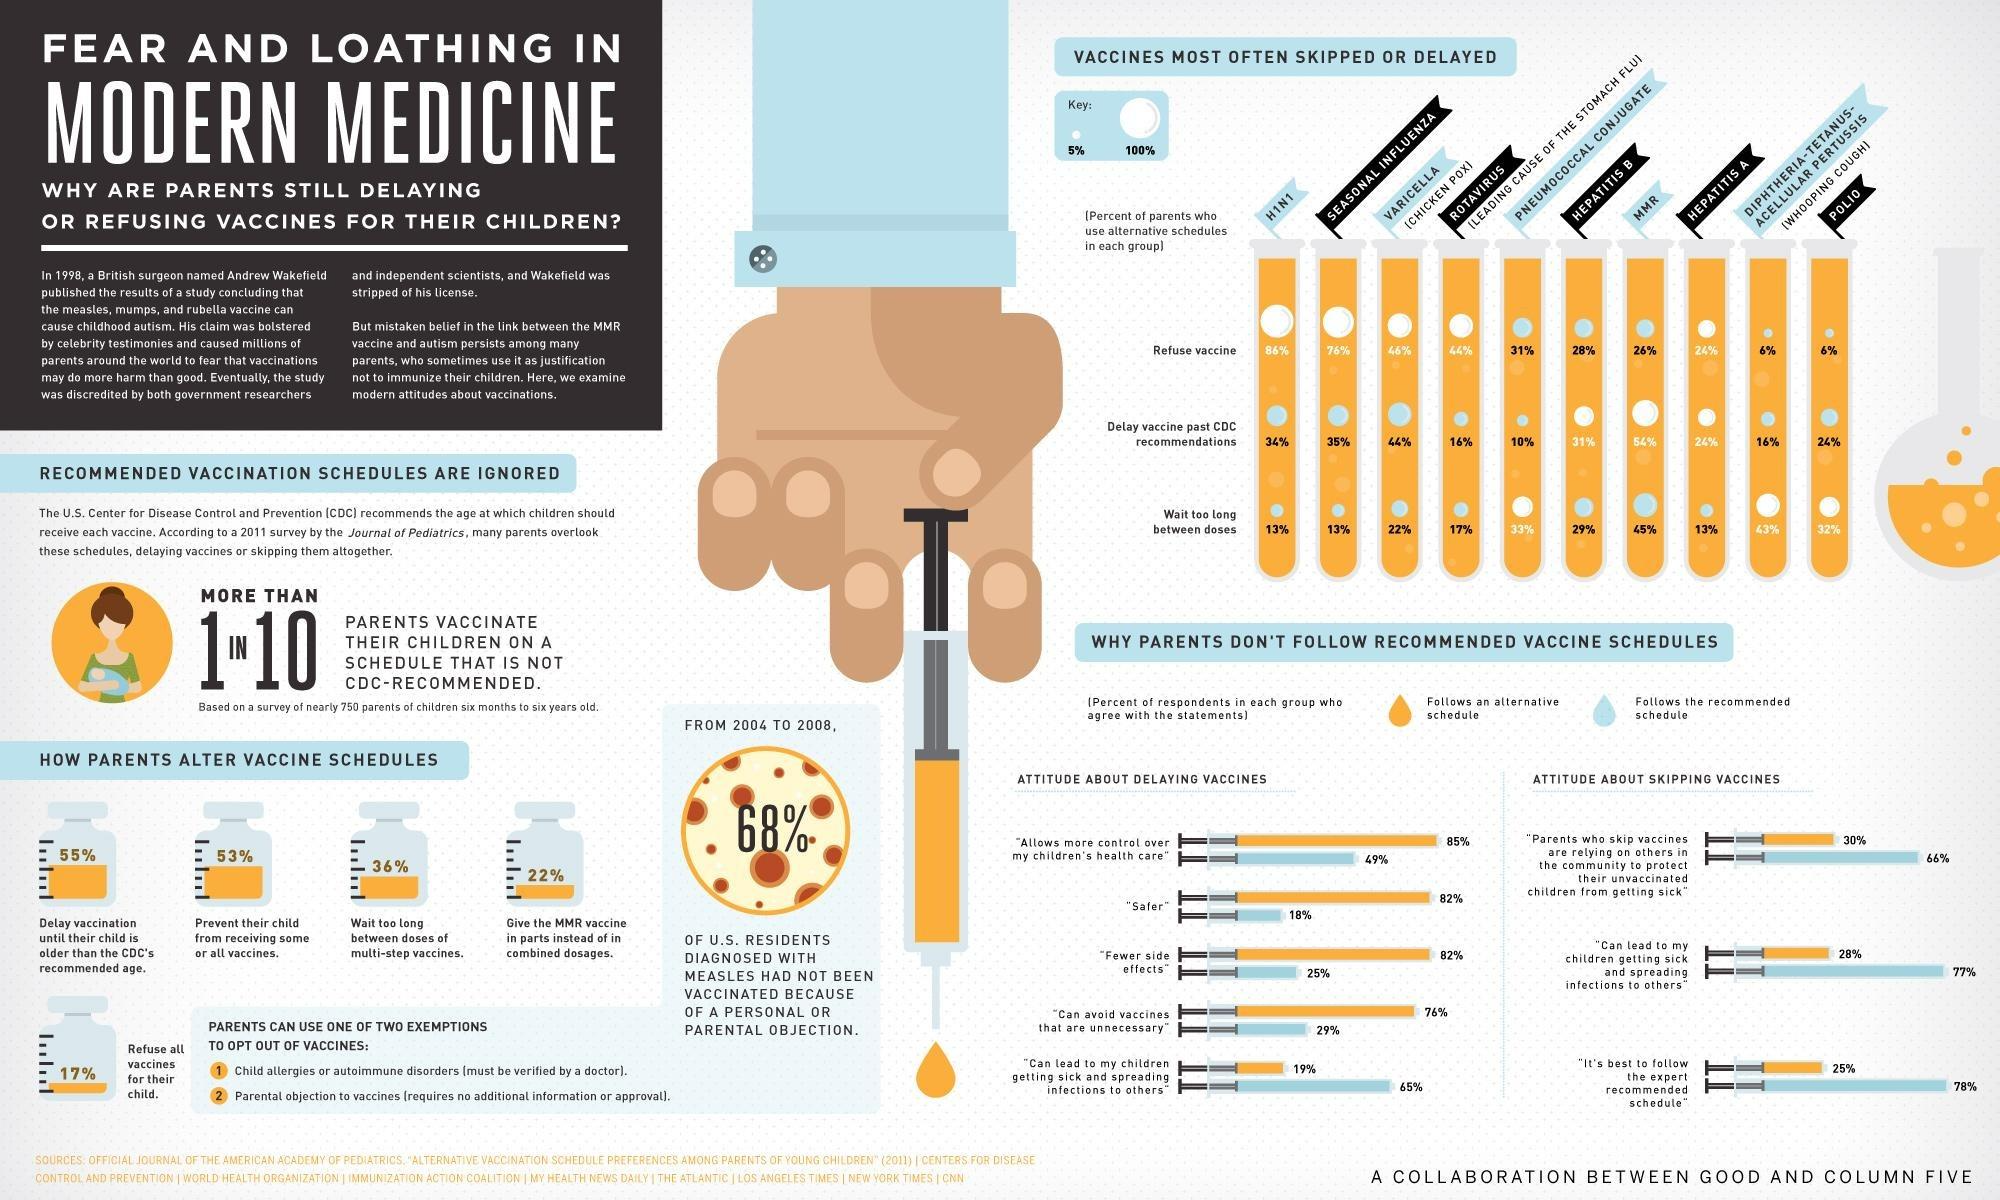
\includegraphics[width=0.99\textwidth]{figures/training_data_examples/10.png} \\[4pt]

\textbf{Image-text Interleaved CoT:}\\
The question asks for the percentage of parents who delay the Varicella vaccine according to CDC recommendations, based on the provided infographic. I need to find the section of the infographic that lists vaccines and the percentages for delaying them past CDC recommendations. I will focus on the Varicella vaccine data.

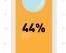
\includegraphics[width=0.12\textwidth]{figures/training_data_examples/11.png} \\[4pt]

The cropped image shows the specific data point for the \verb|<observation>|Varicella vaccine\verb|</observation>| under the \"Delay vaccine past CDC recommendations\" row. Therefore, the final answer is \boxed{44\%}.

\end{tcolorbox}
\caption{\textbf{Example of Monet-SFT-125K: cropping the crucial region.}}
\label{fig:training_data_example1}
\end{figure*}





\begin{figure*}[t]
\centering
\begin{tcolorbox}[title=\textbf{Monet-SFT-125K Example 2: Creating New Visual States (from Zebra-CoT 3D Object Counting)},
    colback=gray!5, colframe=gray!40,
    left=1mm, right=1mm, top=1mm, bottom=1mm,
    enhanced, sharp corners, width=\textwidth]

\textbf{Question:} Consider the initial arrangement of objects presented in the image below. You are required to perform a series of removal operations in the specified order:\\Step 1: Eliminate all objects identified as PYRAMIDs.\\Step 2: Eliminate all objects that are BLUE in color.\\Step 3: Eliminate all objects that are RED in color.\\After completing these steps, determine the total count of orange objects remaining.\\Put your final answer within \verb|\\boxed{}|."
 \\[4pt]

\textbf{Question Image:}\\
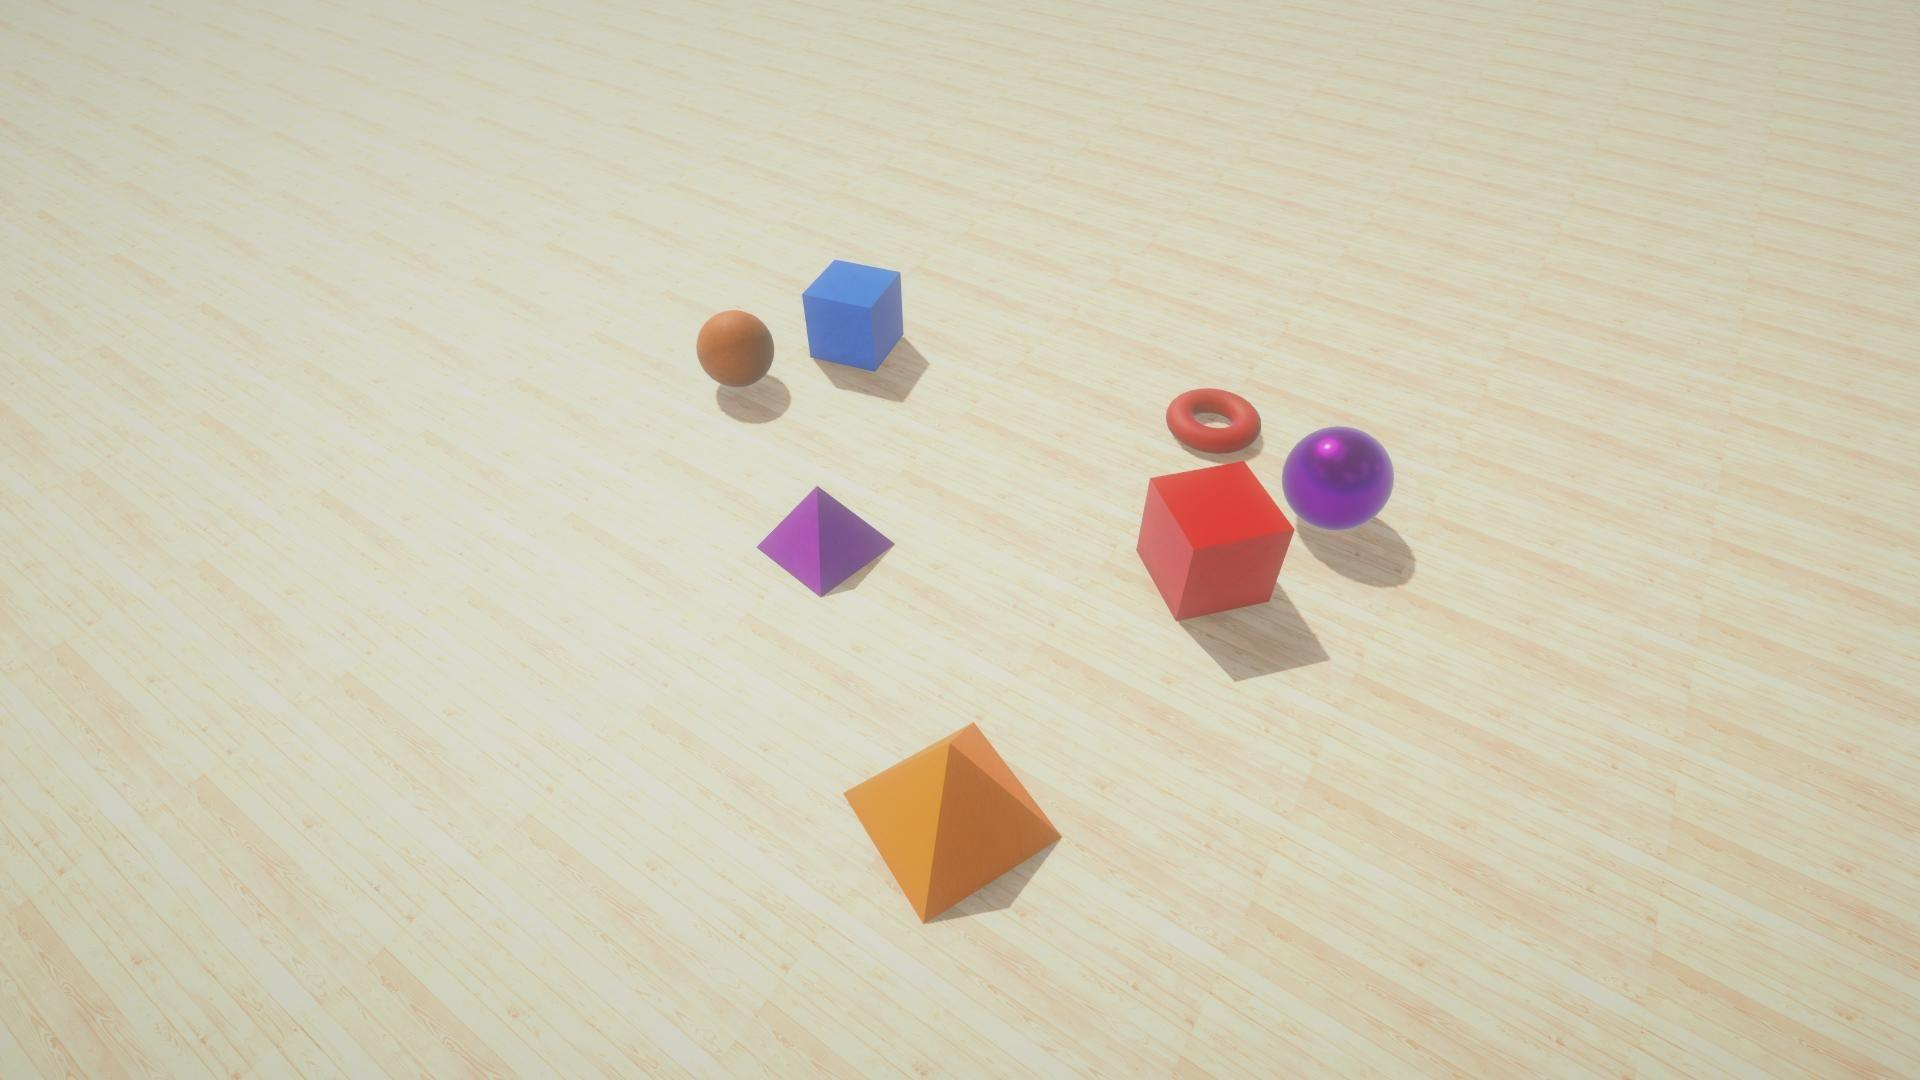
\includegraphics[width=0.27\textwidth]{figures/training_data_examples/1.png} \\[4pt]

\textbf{Image-text Interleaved CoT:}\\
I will begin by analyzing the initial set of objects shown in the problem image. There are \verb|<observation>|7\verb|</observation>| distinct objects in the initial configuration. My approach will be to systematically apply each removal step and visually track the remaining objects before arriving at the final count.
The first operation requires the removal of all pyramid-shaped objects from the scene. This means both the \verb|<observation>|purple pyramid\verb|</observation>| and the \verb|<observation>|orange pyramid\verb|</observation>| will be taken away. To visualize the updated set of objects, I will generate an image reflecting this change.\\[4pt]
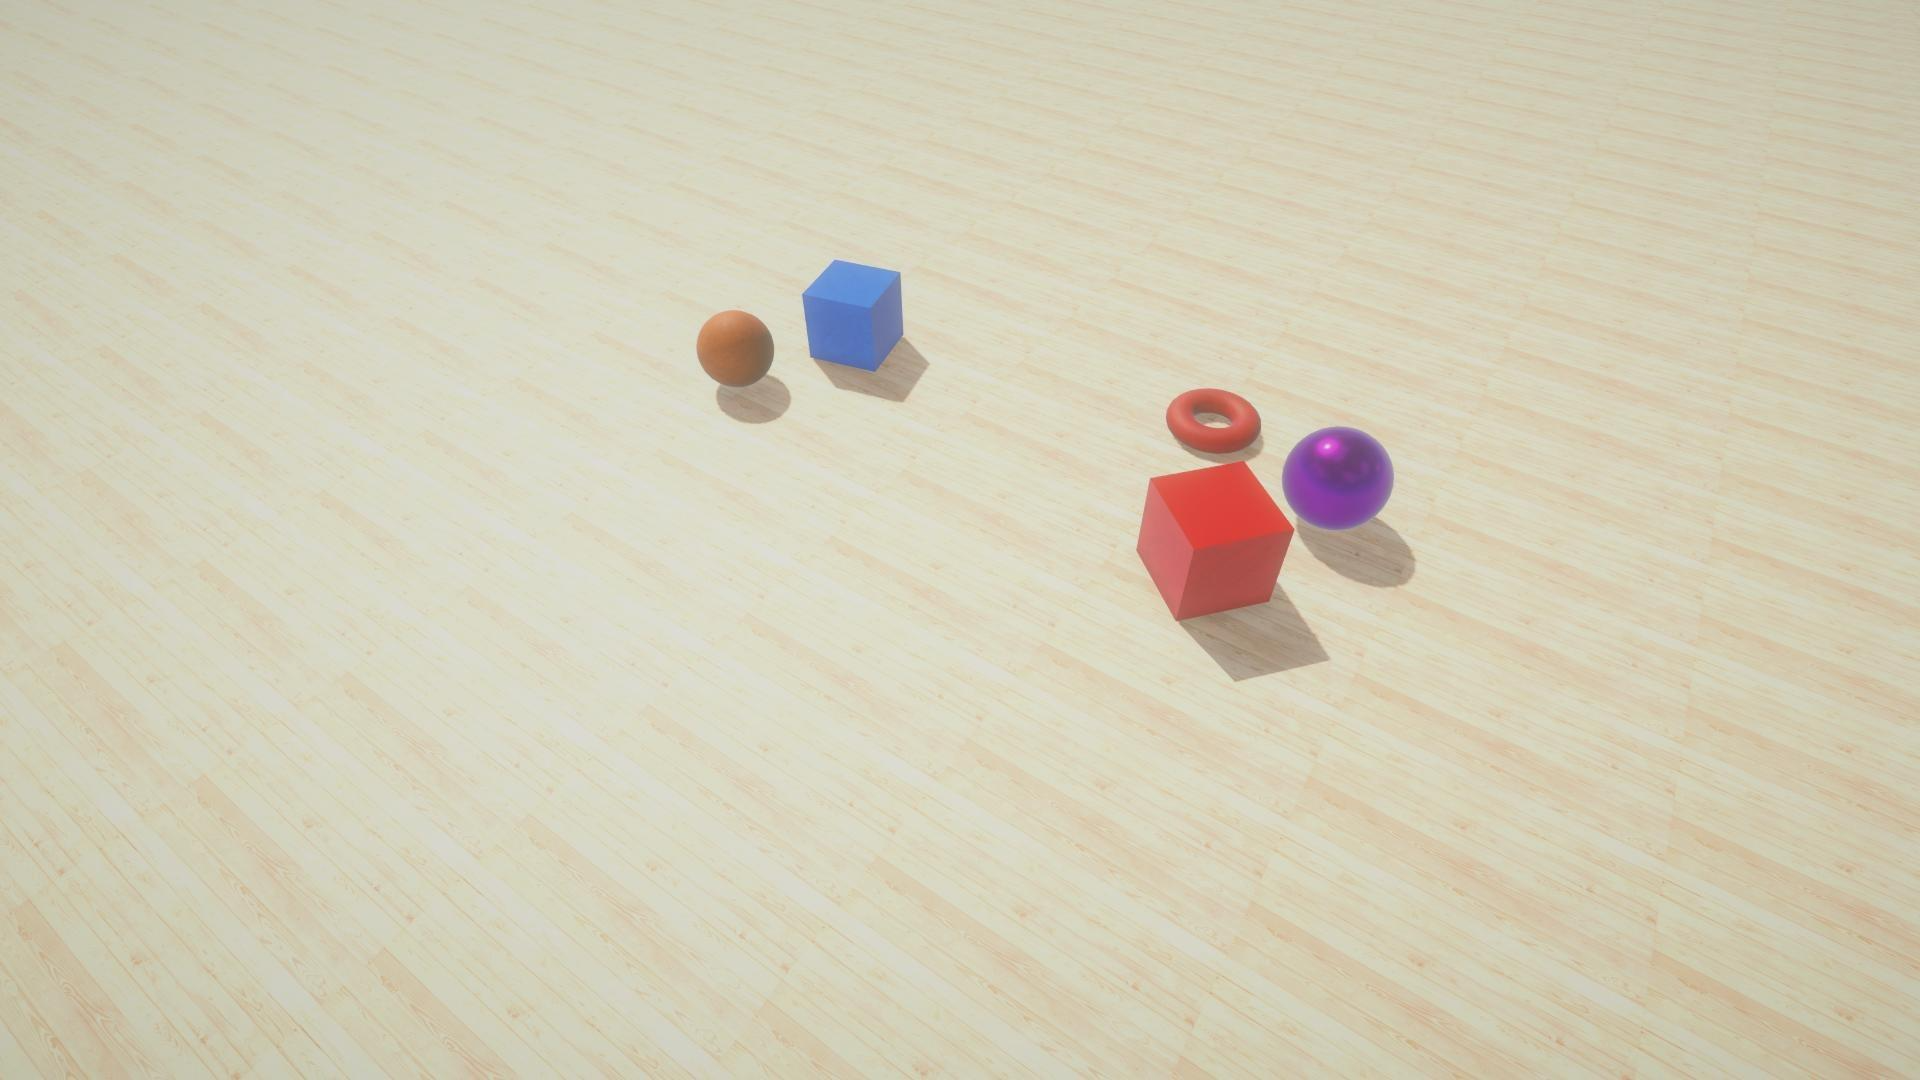
\includegraphics[width=0.27\textwidth]{figures/training_data_examples/2.png} \\[4pt]
After removing the pyramids, as seen in the previous visual, we are left with \verb|<observation>|five\verb|</observation>| objects: an \verb|<observation>|orange sphere\verb|</observation>|, a \verb|<observation>|blue cube\verb|</observation>|, a \verb|<observation>|red torus\verb|</observation>|, a \verb|<observation>|red cube\verb|</observation>|, and a \verb|<observation>|purple sphere\verb|</observation>|. The next instruction is to remove all objects that are blue. This specifically targets the \verb|<observation>|blue cube\verb|</observation>|. I will generate a new visual to show the state after this removal.\\[4pt]
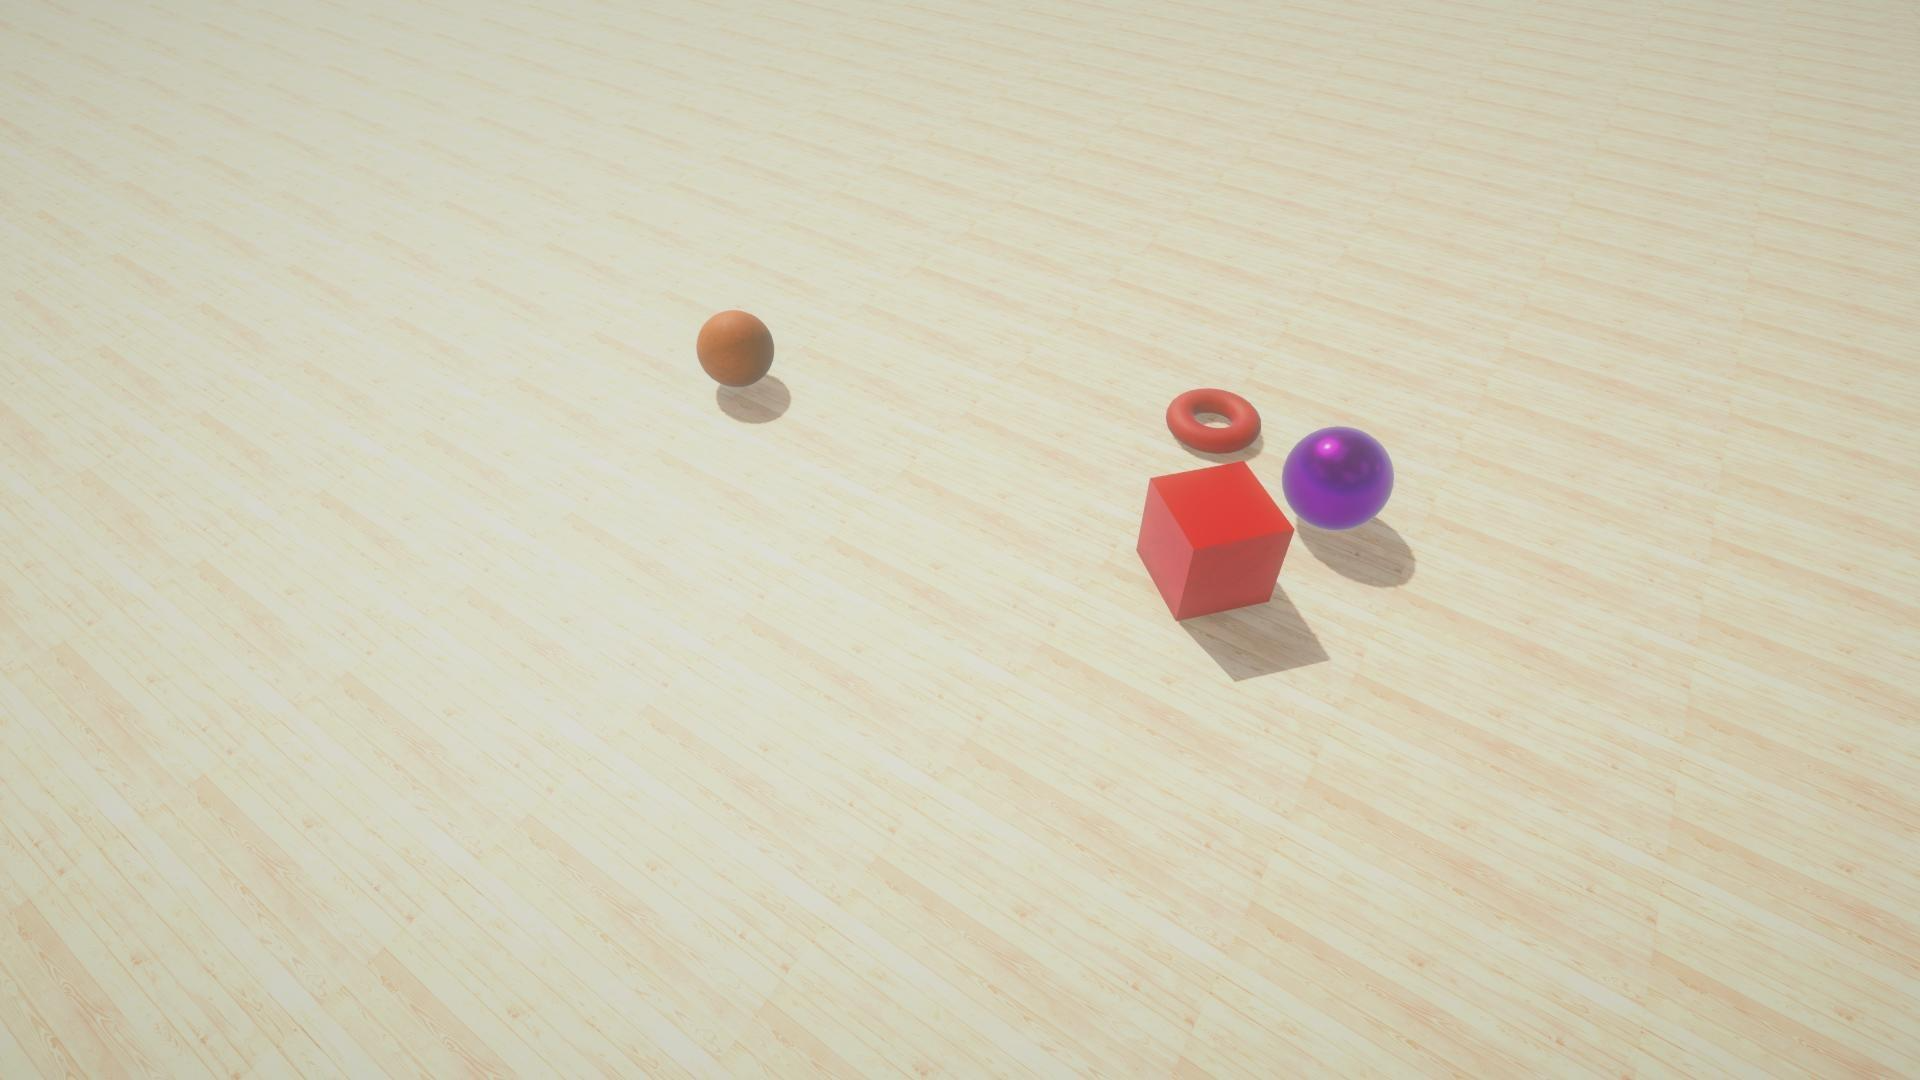
\includegraphics[width=0.27\textwidth]{figures/training_data_examples/3.png} \\[4pt]
...\\[4pt]
Having completed all specified removal operations, the final visual shows \verb|<observation>|two\verb|</observation>| objects remaining: an \verb|<observation>|orange sphere\verb|</observation>| and a \verb|<observation>|purple sphere\verb|</observation>|. The question asks for the count of orange objects. From the two remaining objects, only one is orange. The final answer is \boxed{1}. 
\end{tcolorbox}
\caption{\textbf{Example of Monet-SFT-125K: creating new visual states.}}
\label{fig:training_data_example2}
\end{figure*}







\begin{figure*}[t]
\centering
\begin{tcolorbox}[title=\textbf{Monet-SFT-125K Example 3: Drawing Auxiliary Lines and Bounding Boxes (from CogCoM)},
    colback=gray!5, colframe=gray!40,
    left=1mm, right=1mm, top=1mm, bottom=1mm,
    enhanced, sharp corners, width=\textwidth]

\textbf{Question:}What is the sum of real users below 1 million?\\Put your final answer within \verb|\\boxed{}|."
 \\[4pt]

\textbf{Question Image:}\\
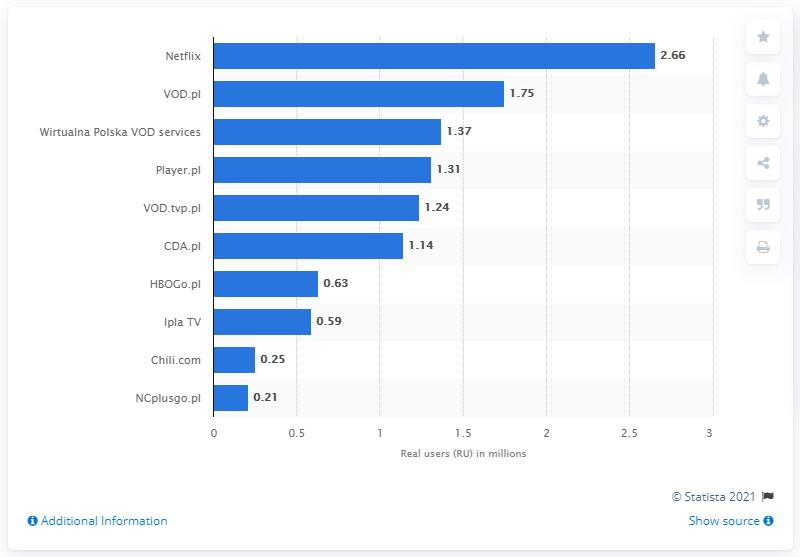
\includegraphics[width=0.3\textwidth]{figures/training_data_examples/5.png} \\[4pt]

\textbf{Image-text Interleaved CoT:}\\
Draw a line to obtain the new image after the line is drawn.\\
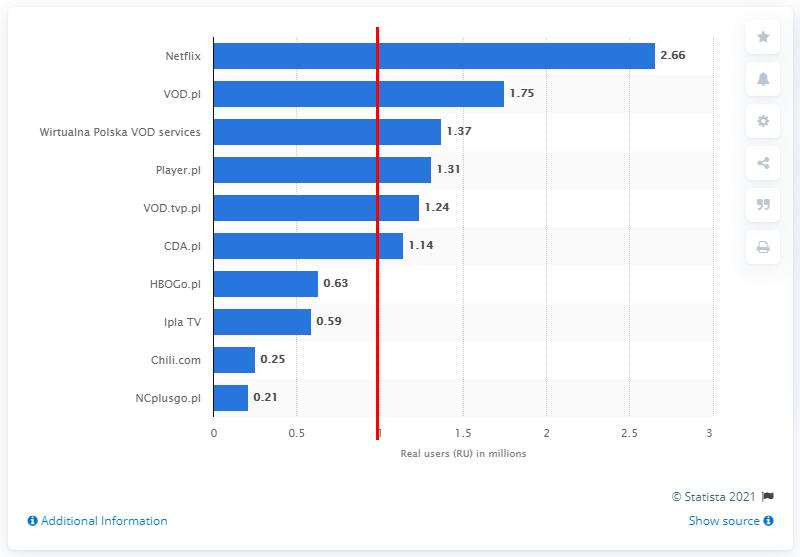
\includegraphics[width=0.3\textwidth]{figures/training_data_examples/6.png} \\[4pt]
Outline each bar column, which are located at Netflix, VoD.pI, Wirtualna Polska VOD services, Player.pl, VoD.tvp.pI, CDA.pI, HBOGo.pI, lpla TV, Chili.com, NCplusgo.pl. \\[4pt]
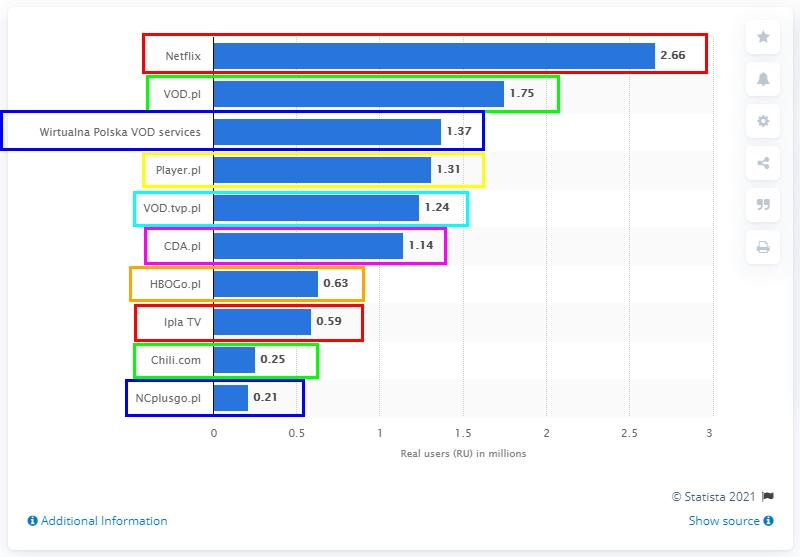
\includegraphics[width=0.3\textwidth]{figures/training_data_examples/7.png} \\[4pt]
Analyze the value of each bar in relation to x=1. The values obtained from HBOGo.pI, lpla TV, Chili.com, and NCplusgo.pl are all \verb|<observation>|less than one million\verb|</observation>|, with respective values of \verb|<observation>|0.63, 0.59, 0.25, and 0.21.\verb|</observation>| Calculate their total sum as 0.63 + 0.59 + 0.25 + 0.21 = 1.68, so the answer is 1.68.
 The final answer is \boxed{1.68}. 
\end{tcolorbox}
\caption{\textbf{Example of Monet-SFT-125K: drawing auxiliary lines and bounding boxes.}}
\label{fig:training_data_example3}
\end{figure*}






















\subsection{Inference Examples}
We present some inference examples generated by Monet-7B in this section to show the generality of tasks that Monet-7B can solve. For clarity, we don't map the generated latent embeddings to the language space as this will produce meaningless tokens. Instead, we use \verb|<latent><latent_embeddings></latent>| to represent the latent reasoning segments.

The tasks of the selected examples include 3D Spatial Reasoning (Figure \ref{fig:inference_example1}), 2D transformation (Figure \ref{fig:inference_example2}), complex diagram reasoning (Figure \ref{fig:inference_example3}), commonsense QA (Figrue \ref{fig:inference_example4}), fine-grained OCR (Figure \ref{fig:inference_example5}), and math reasoning (Figure \ref{fig:inference_example6}). Note that Monet not always uses latent thinking. For example, for the pure-text math problem in Figure \ref{fig:inference_example6}, and Monet directly rely text-based reasoning to solve the problem.







\begin{figure*}[t]
\centering
\begin{tcolorbox}[title=\textbf{Monet-7B Inference Example 1: 3D Spatial Reasoning (from VisualPuzzles)},
    colback=gray!5, colframe=blue!60,
    left=1mm, right=1mm, top=1mm, bottom=1mm,
    enhanced, sharp corners, width=\textwidth]

\textbf{Question:}Given a pair of chairs arranged at a specific angle, select the option from the four provided that matches the angle of the chairs in the question.
Options: Choose from (A) (B) (C) (D) in the image.
"
 \\[4pt]

\textbf{Question Image:}\\
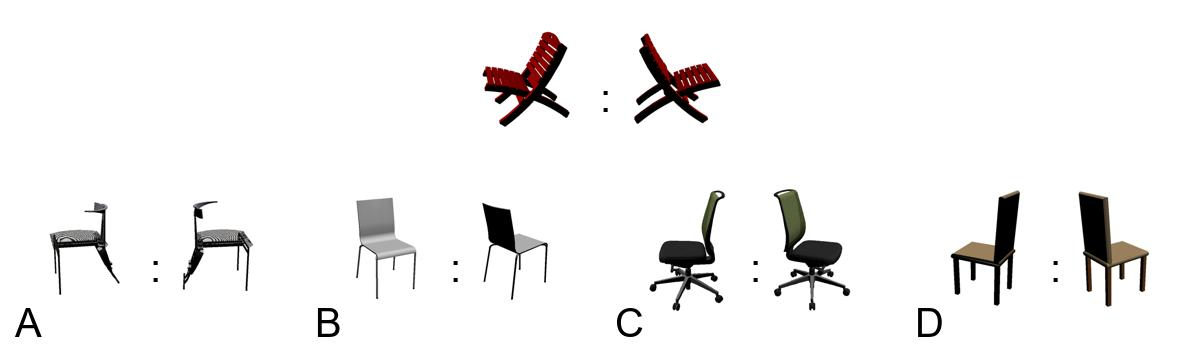
\includegraphics[width=0.6\textwidth]{figures/training_data_examples/19.png} \\[4pt]

\textbf{Response by Monet-7B:}\\
The problem asks to identify the option that matches the given angle between the chairs. I will analyze the provided image to determine the angle between the chairs and then compare it with the given choices.To accurately assess the angle between the chairs, I will focus on the visual representation of the chairs in the problem image.
\verb|<latent><latent_embeddings></latent>|The zoomed-in view of the chairs in the problem image clearly shows the angle between them. This visual confirms the specific spatial relationship between the two chairs. Therefore, the final answer is \boxed{A}.

\end{tcolorbox}
\caption{\textbf{Inference example: 3D spatial reasoning.} Instead of describing the angles between the chairs in language, Monet directly reasons with latent embeddings before giving the final answer.}
\label{fig:inference_example1}
\end{figure*}








\begin{figure*}[t]
\centering
\begin{tcolorbox}[title=\textbf{Monet-7B Inference Example 2: 2D Transformation (from VisualPuzzles)},
    colback=gray!5, colframe=blue!60,
    left=1mm, right=1mm, top=1mm, bottom=1mm,
    enhanced, sharp corners, width=\textwidth]

\textbf{Question:} The number 4 is reflected twice in \verb|<image1>|. Which among the options in \verb|<image2>| should appear in the field with the question mark if we do the same with the number 5?
"
 \\[4pt]

\textbf{Question Image:}\\
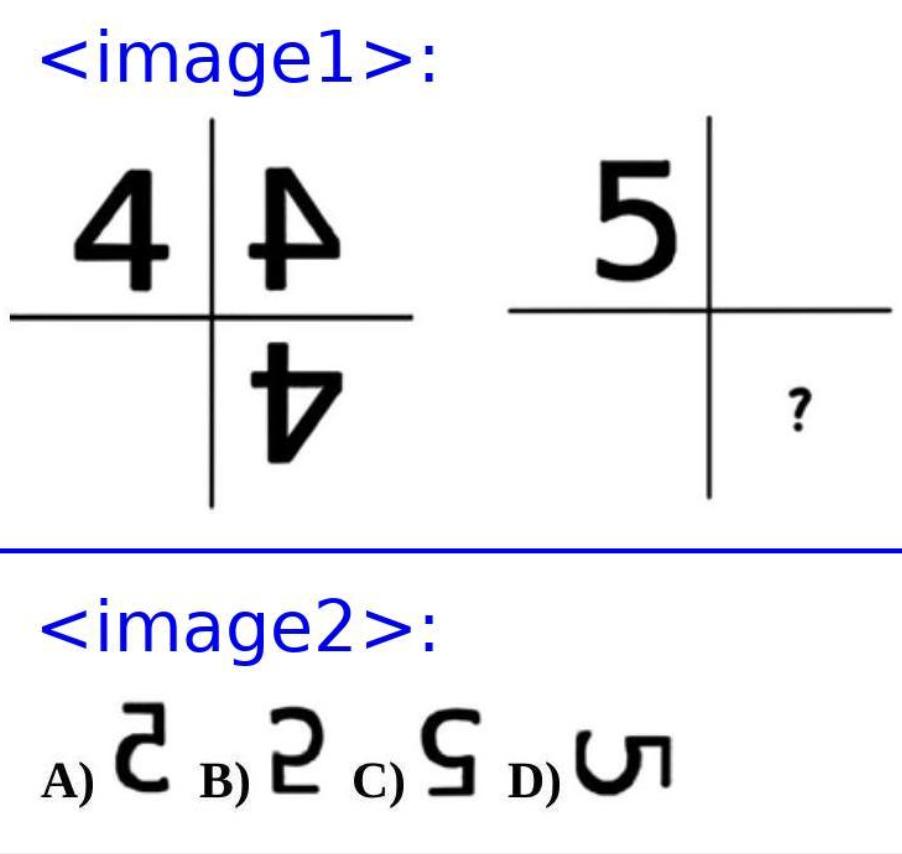
\includegraphics[width=0.5\textwidth]{figures/training_data_examples/20.png} \\[4pt]

\textbf{Response by Monet-7B:}\\
To determine the correct answer, we need to identify the pattern of reflection for the number 5, similar to how the number 4 is reflected in the provided image.To better understand the reflection pattern, I will generate a zoomed-in view of the relevant section of the image.
\verb|<latent><latent_embeddings></latent>|The zoomed-in image clearly shows how number 4 is reflected. The reflection pattern for the number 4 is obtained by flipping it twice. Once horizontally, once vertically. Therefore, the final answer is \boxed{C}.


\end{tcolorbox}
\caption{\textbf{Inference example: 2D transformation.} By generating latent embeddings, Monet successfully identifies the flipping rule of the number.}
\label{fig:inference_example2}
\end{figure*}









\begin{figure*}[t]
\centering
\begin{tcolorbox}[title=\textbf{Monet-7B Inference Example 3: Complex Diagram Reasoning (from MME-RealWorld-Lite)},
    colback=gray!5, colframe=blue!60,
    left=1mm, right=1mm, top=1mm, bottom=1mm,
    enhanced, sharp corners, width=\textwidth]

\textbf{Question:} Which country is the top sales country? The choices are listed below:\\
(A) Canada\\
(B) Germany\\
(C) UK\\
(D) United States\\
(E) The image does not feature the number.
 \\[4pt]

\textbf{Question Image:}\\
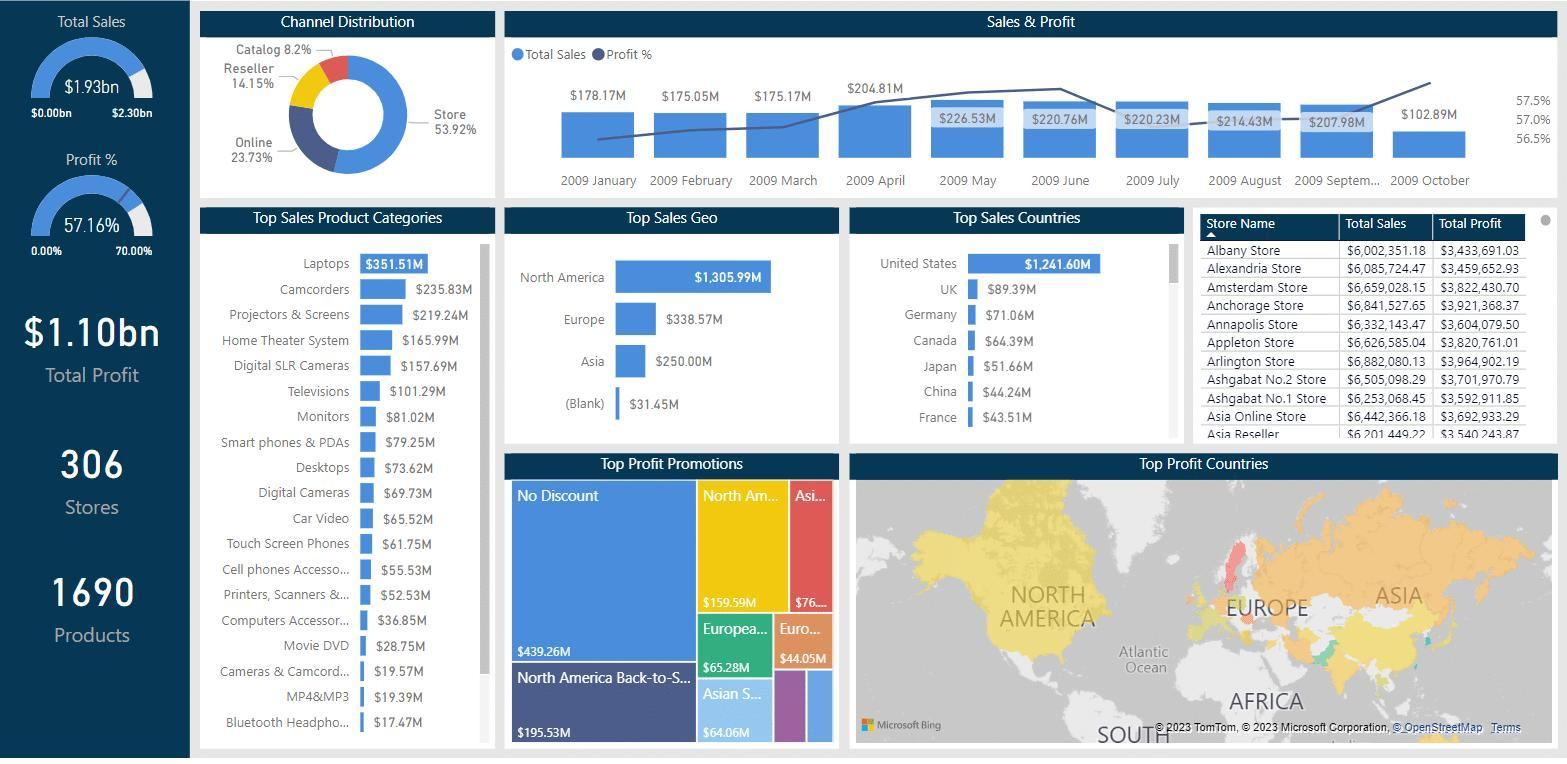
\includegraphics[width=0.99\textwidth]{figures/training_data_examples/21.png} \\[4pt]

\textbf{Response by Monet-7B:}\\
To determine the top sales country, I need to locate the section of the image that displays sales by country.
\verb|<latent><latent_embeddings></latent>|The highlighted area in the image clearly shows the "Top Sales Countries" section. It lists various countries along with their respective sales figures. The sales figures are in millions of dollars.
From the highlighted section, I can see that the United States has the highest sales at 1,241.60M, followed by the UK, Germany, and other countries. This directly answers the question about the top sales country. The final answer is \boxed{D}.



\end{tcolorbox}
\caption{\textbf{Inference example: complex diagram reasoning.} Monet-7B exhibit a \textbf{hierarchical} reasoning pattern. Firstlt, it focus on the relevant section in the image by generating latent embeddings: ``\textit{The highlighted area in the image clearly shows the ``Top Sales Countries" section.}'' Then, it accurately identifies the contents in the ``Top Sales Countries'' section and gives the correct answer.}
\label{fig:inference_example3}
\end{figure*}











\begin{figure*}[t]
\centering
\begin{tcolorbox}[title=\textbf{Monet-7B Inference Example 4: Commonsense QA (from VisualPuzzles)},
    colback=gray!5, colframe=blue!60,
    left=1mm, right=1mm, top=1mm, bottom=1mm,
    enhanced, sharp corners, width=\textwidth]

\textbf{Question:} Based on the relationship between Origin and Analogy, select the option from the candidates that best completes this analogy.\\
Options: Choose from (A) (B) (C) (D) in the image.
 \\[4pt]

\textbf{Question Image:}\\
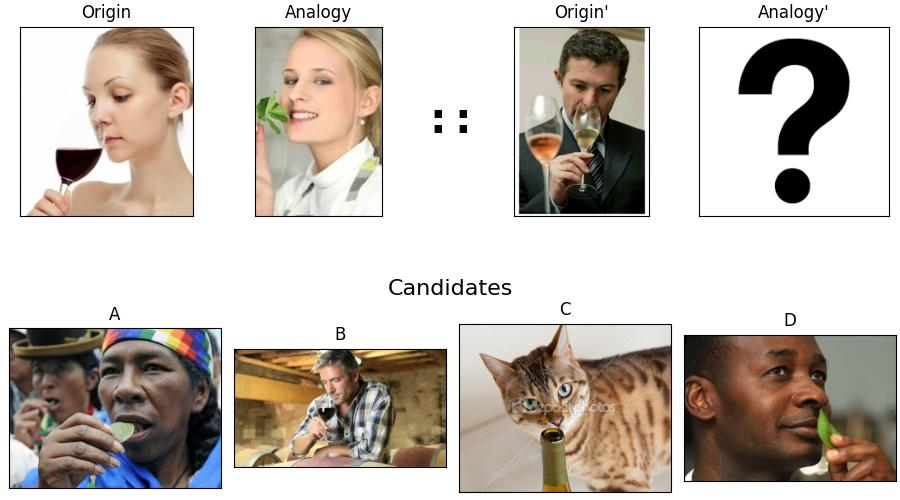
\includegraphics[width=0.99\textwidth]{figures/training_data_examples/22.png} \\[4pt]

\textbf{Response by Monet-7B:}\\
To identify the correct image that completes the analogy, I will analyze the relationship between the "Origin" and "Analogy" images in the provided problem image. The goal is to find a similar relationship between the "Origin'" image and the missing "Analogy'" image. To better understand the relationship, I will focus on the "Origin" and "Analogy" images to identify the specific action being performed by the person in each image. \verb|<latent><latent_embeddings></latent>| \\
The zoomed-in view of the "Origin" image clearly shows  a person  drinking wine, while the "Analogy" image depicts  a person  smelling a flower. This indicates that the action involves the sense of smell.Therefore, the final answer is \boxed{D}.

\end{tcolorbox}
\caption{\textbf{Inference example: commonsense QA.} Monet-7B correctly identifies the connection between the ``Origin'' and the ``Analogy'' image, showing its commonsense reasoning capability.}
\label{fig:inference_example4}
\end{figure*}





\begin{figure*}[t]
\centering
\begin{tcolorbox}[title=\textbf{Monet-7B Inference Example 5: Fine-grained OCR (from MME-RealWorld-Lite)},
    colback=gray!5, colframe=blue!60,
    left=1mm, right=1mm, top=1mm, bottom=1mm,
    enhanced, sharp corners, width=\textwidth]

\textbf{Question:} Where does Joseph work? The choices are listed below:\\
(A) Boston.\\
(B) Miami.\\
(C) Chicago.\\
(D) New York.\\
(E) The image does not feature the related information.
 \\[4pt]

\textbf{Question Image:}\\
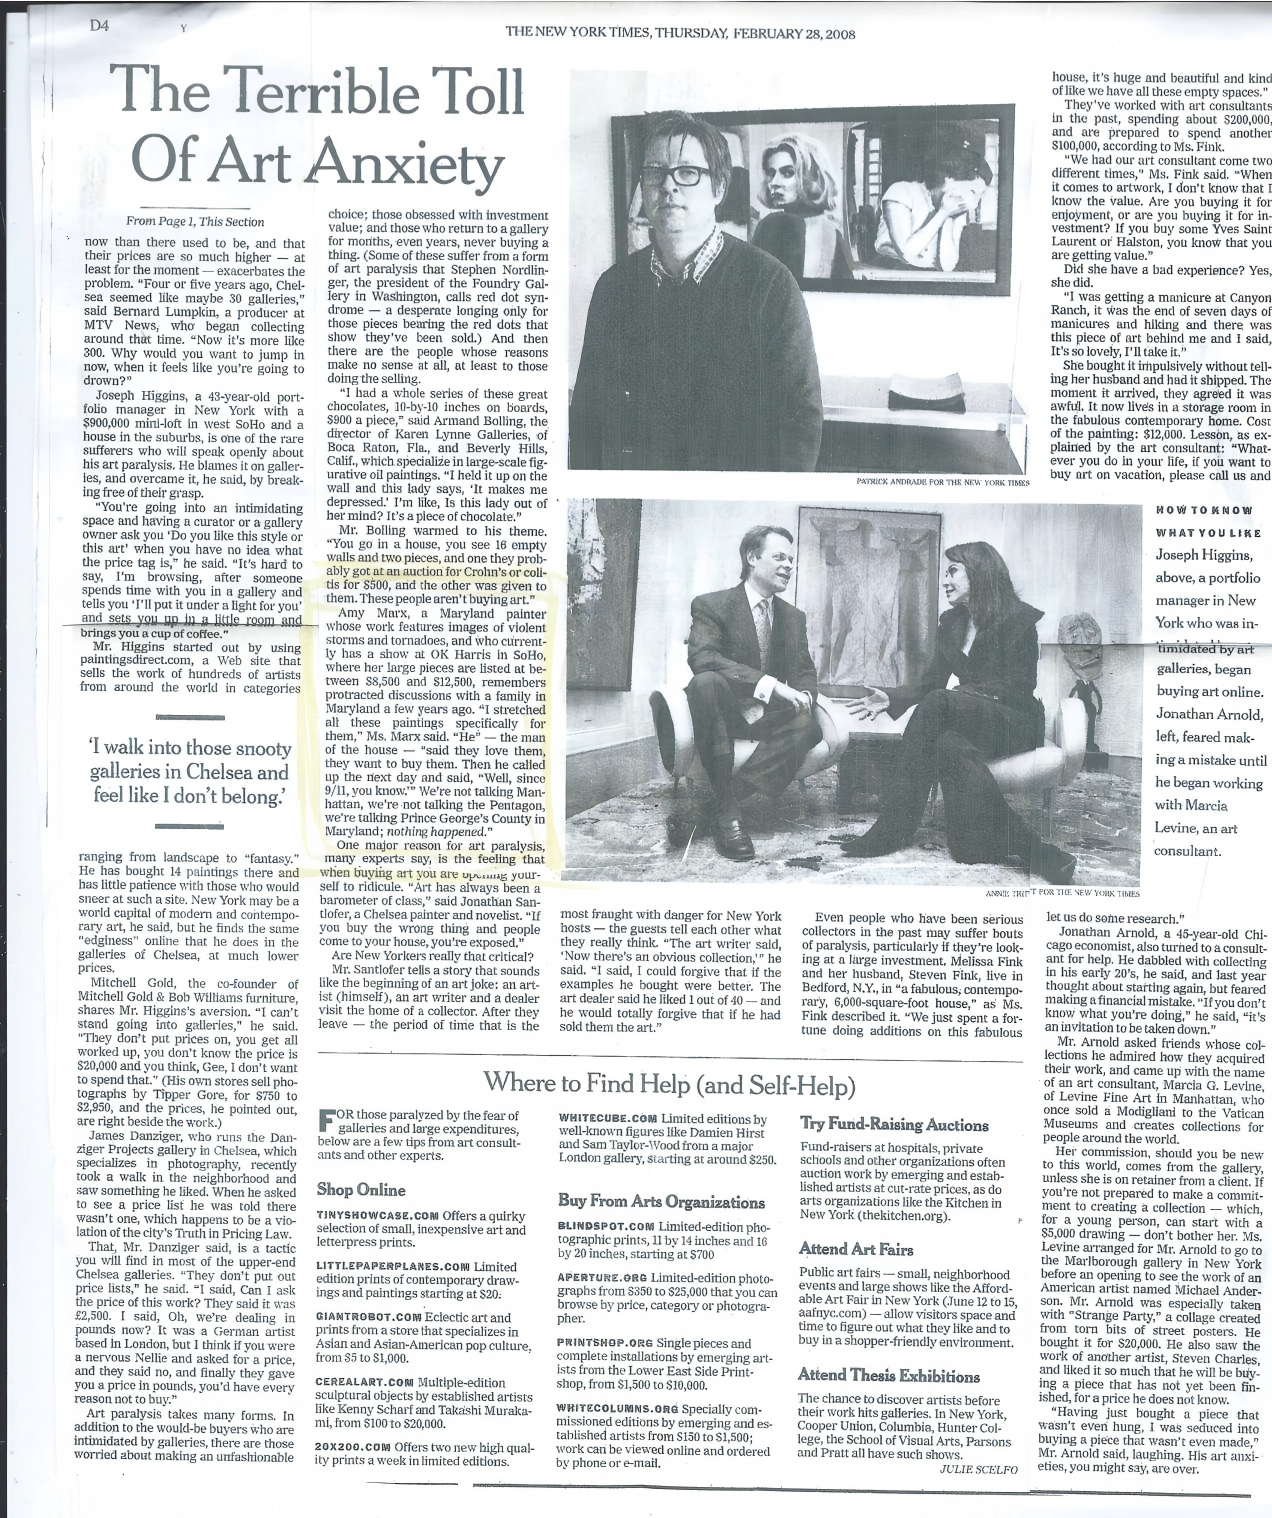
\includegraphics[width=0.7\textwidth]{figures/training_data_examples/23.png} \\[4pt]

\textbf{Response by Monet-7B:}\\
To determine where Joseph works, I need to locate his name or relevant information within the article. I will zoom in on the section of the article that mentions Joseph to clearly identify his location. \verb|<latent><latent_embeddings></latent>| \\
The zoomed-in image clearly shows that Joseph Higgins is a portfolio manager in  New York. This directly answers the question about where Joseph works.Therefore, the final answer is \boxed{D}.


\end{tcolorbox}
\caption{\textbf{Inference example: fine-grained OCR.} Monet-7B accurately identifies the key information, which is located in the middle of the rightmost region of the image.}
\label{fig:inference_example5}
\end{figure*}







\begin{figure*}[t]
\centering
\begin{tcolorbox}[title=\textbf{Monet-7B Inference Example 6: Math Reasoning (from VisualPuzzles)},
    colback=gray!5, colframe=blue!60,
    left=1mm, right=1mm, top=1mm, bottom=1mm,
    enhanced, sharp corners, width=\textwidth]

\textbf{Question:} Every night the wizard Tilim makes the weather forecast for the king. When Tilim gets it right he gets 3 gold coins, but when he makes a mistake, he pays a fine of 2 gold coins. After making the prediction for 5 days, Tilim did the math and discovered that he neither won nor lost coins. How many times did he get the weather forecast right in those 5 days?\\                             Options:\\                                                                                                                                (A) 1\\
(B) 2\\
(C) 3\\
(D) 4\\[4pt]


\textbf{Response by Monet-7B:}\\
To determine the number of correct weather forecasts, we can set up an equation based on the given conditions. Let's define:               - \( x \) as the number of correct forecasts (where he earns 3 gold coins per correct forecast).\\
- \( y \) as the number of incorrect forecasts (where he loses 2 gold coins per incorrect forecast)\\
The wizard made a total of 5 forecasts, so:\\
\[ x + y = 5 \]\\
He neither won nor lost any gold, which means the total gain from correct forecasts equals the total loss from incorrect forecasts: \[ 3x = 2y \]We now have a system of two equations:\\
1. \( x + y = 5 \)\\
2. \( 3x = 2y \)\\
We can solve this system by expressing \( y \) in terms of \( x \) from the first equation:\[ y = 5 - x \]Next, substitute \( y = 5 - x \) into the second equation:\[ 3x = 2(5 - x) \]Solve for \( x \):\[ 3x = 10 - 2x \]\[ 3x + 2x = 10 \]\[ 5x = 10 \]\[ x = 2 \]So, Tilim made 2 correct forecasts. To verify, we calculate \( y \):\[ y = 5 - x = 5 - 2 = 3 \]Now, check the total gold:\\
- Correct forecasts: \( 2 \times 3 = 6 \) gold\\
- Incorrect forecasts: \( 3 \times (-2) = -6 \) gold\\
- Total gold: \( 6 + (-6) = 0 \) gold. The calculations confirm that Tilim neither won nor lost any gold. Therefore, the number of correct forecasts is \boxed{2}. The final answer is \boxed{B}.


\end{tcolorbox}
\caption{\textbf{Inference example: math reasoning.} Monet-7B can perform pure-text math reasoning. Since the problem is not visual-related, it doesn't activate latent thinking mode.}
\label{fig:inference_example6}
\end{figure*}